\documentclass{article}
\usepackage{xeCJK}
\usepackage{amsmath,esint,amssymb}
\usepackage{hyperref}
\usepackage{graphicx}
\usepackage{bm}
\DeclareMathOperator*{\rgmax}{argmax}
\DeclareMathOperator{\Var}{Var}
\begin{document}
\title{第三章作业}
\author{赵丰,2017310711}
\maketitle
\textbf{P1}
观测$y(n)=x(n)+w(n)$,$w(n)$是高斯白噪声。
$r_y(0)=5+r_x(0)=15,r_y(1)=r_x(1)=5$,
又$r_{xy}(0)=r_x(0),r_{xy}(1)=r_x(1)$
解Wiener-Hopf方程:
\begin{equation}
\begin{bmatrix}
r_y(0) & r_y(1)\\
r_y(1) & r_y(0)\\
\end{bmatrix}\binom{w_1}{w_2}=
\binom{r_{xy}(0)}{r_{xy}(1)}
\end{equation}
解得$w_1=0.625,w_2=0.125$
由最优滤波器的均方误差公式:
\begin{equation}
J_{\text{min}}=\sigma_x^2-r_{yx}^T \bm{w}
\end{equation}
得到均方误差为$3.125$。

\textbf{P2}
欲极小化$E((d(n)-x(n)-w_1 x(n-1))^2)$
\begin{equation}
E((d(n)-x(n)-w_1 x(n-1))^2)=\sigma_d^2+(1+w_1^2)r_x(0)-2r_{xd}(0)-2w_1r_{xd}(-1)+2w_1r_x(1)
\end{equation}
上式对$w_1$求导并令导数等于零解得:
\begin{equation}
w_1=\frac{r_{xd}(-1)-r_x(1)}{r_x(0)}=0.5
\end{equation}
最小均方误差为$E((d(n)-x(n)-0.5 x(n-1))^2)=6.75$

\textbf{P4(1)}
针对2系数的FIR型滤波器,$r_x(0)=r_s(0)+\sigma_w^2,r_x(1)=r_s(1)$
由AR(1)过程的自相关函数公式$r_s(n)=\frac{\sigma_v^2}{1-\alpha^2}\alpha^{|n|}$,
因此:$r_x(0)=\frac{\sigma_v^2}{1-\alpha^2}+\sigma_w^2$,$r_x(1)=\frac{\sigma_v^2 \alpha}{1-\alpha^2}$
设$d(n)=s(n+K)$,则
$r_{xd}(0)=r_s(K)$,$r_{xd}(-1)=r_s(K+1)$
因此方程组为
\begin{equation}
\begin{bmatrix}
\frac{\sigma_v^2}{1-\alpha^2}+\sigma_w^2 & \frac{\sigma_v^2 \alpha}{1-\alpha^2}\\
\frac{\sigma_v^2 \alpha}{1-\alpha^2} & \frac{\sigma_v^2}{1-\alpha^2}+\sigma_w^2\\
\end{bmatrix}\binom{w_1}{w_2}=
\binom{\frac{\sigma_v^2}{1-\alpha^2}\alpha^{|K|}}{\frac{\sigma_v^2}{1-\alpha^2}\alpha^{|K+1|}}
\end{equation}

\textbf{P4(2)}
代入数据:
\begin{table}[!ht]
\centering
\begin{tabular}{ccc}
\hline
&权系数 & 最小均方误差 \\
\hline
$K=0$ & [0.595238, 0.238095] & 0.595238 \\
$K=1$ & [0.47619, 0.190476] &  1.38095 \\
\hline
\end{tabular}
\end{table}

\textbf{P4(3)}
\begin{equation}
S_x(z)=\sigma_w^2+S_s(z)=\sigma_w^2+\frac{\sigma_v^2}{(1-\alpha z^{-1})(1-\alpha z)}
\end{equation}
因为$r_{dx}(k)=E(d(n)x(n-k))=E(s(n+K)s(n-k))=r_s(K+k)$,所以
\begin{equation}
S_{dx}(z)=z^K S_s(z) =\frac{\sigma_v^2 z^K}{(1-\alpha z^{-1})(1-\alpha z)}
\end{equation}
所以
\begin{equation}
W(z)=\frac{S_{dx}(z)}{S_x(z)}=\frac{\sigma_v^2 z^K}{\sigma_w^2(1-\alpha z^{-1})(1-\alpha z)+\sigma_v^2}
\end{equation}

\textbf{P4(4)}
代入题中参数$W(z)$分母化为$2.64-0.8(z+z^{-1})$
设$2.64-0.8(z+z^{-1})=Q(1-\beta z)(1-\beta z^{-1})$,得方程组$Q\beta=0.8,Q(1+\beta^2)=2.64$,是关于$\beta$的一元二次方程。
取$|\beta|<1$的解有$\beta=0.33756,Q=2.36995$
上式做双边逆Z变换得权系数表达式:
\begin{equation}
w(k)=\frac{1}{Q(1-\beta^2)}\beta^{|k+K|}=0.476(0.34)^{|k+K|}
\end{equation}
分别代入$K=0,K=1$到上式即得非因果型 IIR滤波器的权系数。
对于IIR滤波器,最小均方误差公式为:
\begin{align} 
J_{\text{min}}=& \sigma_d^2-\sum_{l=-\infty}^{\infty} w(l) r_{dx}(l)\\
 =&\sigma_d^2-\sum_{l=-\infty}^{\infty} \frac{1}{Q(1-\beta^2)}\beta^{|l+K|} r_{s}(l+K)\\
 =&\sigma_d^2-\sum_{l=-\infty}^{\infty} \frac{1}{Q(1-\beta^2)}\beta^{|l|} r_{s}(l)\\
 =&\frac{\sigma_v^2}{1-\alpha^2}\left(1-\sum_{l=-\infty}^{\infty} \frac{1}{Q(1-\beta^2)}\beta^{|l|} \alpha^{|l|}\right)\\
 =&\frac{\sigma_v^2}{1-\alpha^2}\left(1-\frac{1}{Q(1-\beta^2)}(-1+\frac{2}{1-\alpha\beta})\right)
 \end{align}
 得最小均方误差为$0.476$,与$K$无关。
 
 \textbf{P8(1)}
 
 对于一阶最优前向一步预测器,由$r_x(0)w=r_x(-1)$解得权系数$w=0.4$,即$\hat{x}(n)=0.4x(n-1)$,
 预测误差功率为$p_1=r_x(0)-wr_x(-1)=1.17$
 对于二阶最优前向一步预测器,解下面的方程:
\begin{equation}
\begin{bmatrix}
r_x(0) & r_x(1)\\
r_x(1) & r_x(0)\\
\end{bmatrix}\binom{w_1}{w_2}=
\binom{r_{x}(-1)}{r_{x}(-2)}
\end{equation}
得权函数$w_1=0.48,w_2=-0.19$,即$\hat{x}(n)=0.48x(n-1)-0.19x(n-2)$
预测误差功率为$p_2=r_x(0)-r_x(-1)w_1-r_x(-2)w_2=1.01$
\textbf{P8(2)}
3阶前向预测误差滤波器为
 \begin{equation}
f_3(n)=x(n)-w_{f,1}x(n-1)-w_{f,2}x(n-2)-w_{f,3}x(n-3) 
\end{equation}
根据第一问的结果,$a_{2,0}=1,a_{2,1}=-0.48,a_{2,2}=0.19$
直接先计算$\Delta_2=r(-3)a_{2,0}+r(-2)a_{2,1}+r(-1)a_{2,2}=0.095$,
因此三阶反射系数为$k_3=-\frac{\Delta_2}{p_2}=-0.094$
由递推公式
\begin{equation}
a_{m,l}=a_{m-1,l}+k_m a_{m-1,m-l}
\end{equation}
得到$a_{3,1}=a_{2,1}+k_3 a_{2,2}=-0.494$等,与直接解Y-W方程结果一致。
同理可计算出前两阶反射系数为:
$k_1=-\frac{r_x(1)}{r_x(0)}=-0.4$,$k_2=-\frac{\Delta_1}{p_1}=0.171$,


\textbf{P9(1)}
$H_1$与$H_2$级联,输出为AR(2)过程,满足: 
\begin{equation}
x(n)-1.3x(n-1)+0.4x(n-2)=w(n)
\end{equation}
由Wiener-Hopf方程
\begin{align*}
r_x(0)-1.3r_x(1)+0.4r_x(2)= & \sigma_w^2 \\
r_x(1)-1.3r_x(0)+0.4r_x(1)= & 0 \\
r_x(2)-1.3r_x(1)+0.4r_x(0)= & 0
\end{align*}
解得 $r_x(0)=8.64,r_x(1)=8.02,r_x(2)=6.98$

\textbf{P9(2)}
使用2阶预测即可达到最优格型预测误差滤波器的效果。
为设计格型滤波器,只需确定前两阶反射系数。
$k_1=-\frac{r_x(1)}{r_x(0)}=-0.929$,$k_2=-\frac{\Delta_1}{p_1}=0.4$。
系统的结构图如下:
\begin{figure}[!ht]
 \centering
 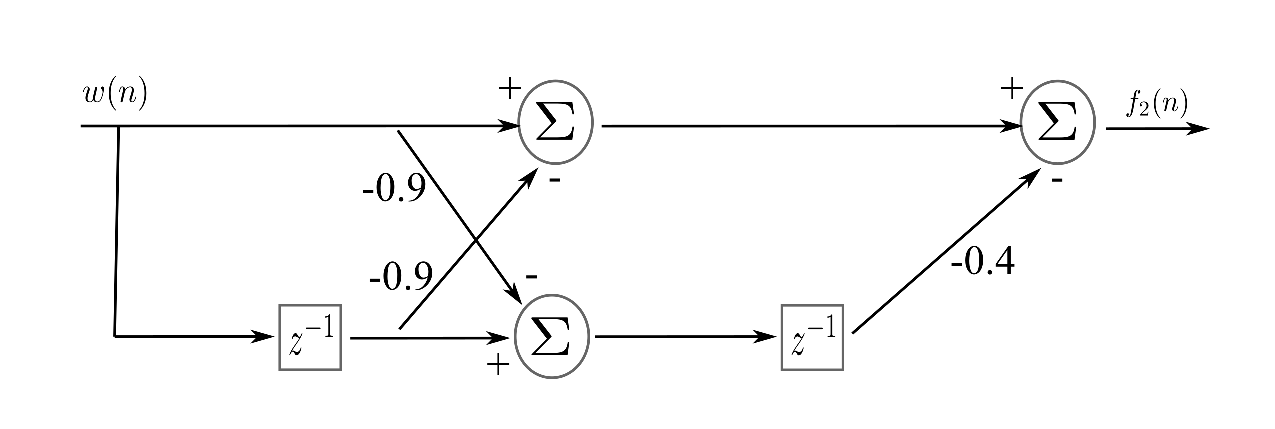
\includegraphics[width=8cm]{gridFilter.eps}
 \caption{两级格型FIR滤波器}
\end{figure}

\textbf{P10}
$e(n)=\displaystyle\sum_{k=-\infty}^{\infty} w^*(k)x(n-k)-d(n)=(w*x)(n)-d(n)$
记$\hat{d}=w*x$,则$e(n)=\hat{d}(n)-d(n)$,
由正交性原理$e(n)$与$x(m),\forall m$正交,因此和$x(m)$的线性组合$\hat{d}$正交。
\begin{align}
r_e(n)=&E(e(m)e(m-n))\\
=& E((\hat{d}(m)-d(m))e(m-n)) \\
=& E(-d(m)e(m-n)) \\
=&r_d(n)-r_{\hat{d}d}(n)\label{eq:hatdd}\\
=&r_d(n)-(w*r_{xd})(n)\label{eq:xd}
\end{align}
其中从\eqref{eq:hatdd}到\eqref{eq:xd}式用到了卷积和期望的线性运算的性质。
上式两边同时做Fourier变换得:
\begin{equation}
S_e(\omega)=S_d(\omega)-W^*(\omega)S_{dx}(\omega)
\end{equation}
由非因果型Wiener滤波器的特点可知,$W(z)=\frac{S_{dx}(z)}{S_x(z)}$
由于功率谱密度的积分与随机过程的方差相等,所以有
\begin{align}
E\{|e(n)|^2\}=& \frac{1}{2\pi}\int_{-\pi}^{\pi}(S_d(\omega)-
\frac{|S_{dx}(\omega)|^2}{S_x(\omega)}) d\omega \\
=& \frac{1}{2\pi}\int_{-\pi}^{\pi}(1-
|C_{dx}(\omega)|^2)S_d(\omega) d\omega
\end{align}


\textbf{P11}
\begin{align}
f_{m-1}(n)=&\sum_{k=0}^{m-1} a_{m-1,k}x(n-k)\\
b_{m-1}(n-1)=&\sum_{k=0}^{m-1} a_{m-1,m-1-k}x(n-1-k)\\
\end{align}
由正交性原理,前向预测误差$f_{m-1}(n)$与$x(n-1),\dots,x(n-m+1)$正交(乘积期望值为0),
所以
\begin{align}
E(f_{m-1}(n)b_{m-1}(n-1))=&a_{m-1,0}\sum_{k=0}^{m-1} a_{m-1,k}E(x(n-k)x(n-m))\\
=& \sum_{k=0}^{m-1} a_{m-1,k}r_x(k-m),a_{m-1,0}=1\\
=& \Delta_{m-1}
\end{align}

\textbf{P13(1)}

\begin{equation}
b_{m}(n)=\sum_{k=0}^{m} a_{m,m-k}x(n-k)\\
\end{equation}
当$i\neq m$时,不妨设$i>m$,则$b_i(n)$与$x(n-m),x(n-m+1),\dots,x(n)$正交(共轭乘积期望值为0),
所以$E(b_m(n)b_i^*(n))=0$,当$i=m$时,由预测误差功率的定义有$E(b_m(n)b_m^*(n))=p_m$。

\textbf{P13(2)}
不访设$i\geq m$,因为$f_i(n)$与$x(n-1),\dots,x(n-i)$正交,所以
\begin{equation}
E[f_m(n)f_i^*(n)]=E[x(n)f_i^*(n)]=E[f_i(n)f_i^*(n)]=p_i
\end{equation}

\textbf{P13(3)}
若$i>j$,因为$k\geq 1$,$f_i(n)$与$x(n-k)$正交,因为$k<i-j$,所以$f_i(n)$与$x(n-k-j)$正交,
即$f_i(n)$与$x(n-k),x(n-k-1),\dots,x(n-k-j)$正交,$f_i(n)$与$f_j(n-k)=\sum_{r=0}^{j} x(n-k-r)$正交,期望值为零。
$i<j$时,由于$n$只是求和指标,可换成$n+k$,将$-k$看成一个整体,$1\leq -k \leq j-i$,
则由刚才证明的式子有$E[f_j(n)f_i^*(n-(-k))]=0$

对于第二式,若$i>j$,序列$x(n-k-j),x(n-k-j+1),\dots,x(n-k)$包含在$x(n-i+1),\dots,x(n)$之间,
所以$b_i(n)$与$x(n-k-j),x(n-k-j+1),\dots,x(n-k)$均正交,即有$b_i(n)$与$b_j(n-k)$正交。同理可证$i<j$。



\begin{equation}
\end{equation}

\end{document}
